\documentclass[]{elsarticle} %review=doublespace preprint=single 5p=2 column
%%% Begin My package additions %%%%%%%%%%%%%%%%%%%

\usepackage[hyphens]{url}

  \journal{Scientific Reports} % Sets Journal name

\usepackage{graphicx}
%%%%%%%%%%%%%%%% end my additions to header

\usepackage[T1]{fontenc}
\usepackage{lmodern}
\usepackage{amssymb,amsmath}
% TODO: Currently lineno needs to be loaded after amsmath because of conflict
% https://github.com/latex-lineno/lineno/issues/5
\usepackage{lineno} % add
\usepackage{ifxetex,ifluatex}
\usepackage{fixltx2e} % provides \textsubscript
% use upquote if available, for straight quotes in verbatim environments
\IfFileExists{upquote.sty}{\usepackage{upquote}}{}
\ifnum 0\ifxetex 1\fi\ifluatex 1\fi=0 % if pdftex
  \usepackage[utf8]{inputenc}
\else % if luatex or xelatex
  \usepackage{fontspec}
  \ifxetex
    \usepackage{xltxtra,xunicode}
  \fi
  \defaultfontfeatures{Mapping=tex-text,Scale=MatchLowercase}
  \newcommand{\euro}{€}
\fi
% use microtype if available
\IfFileExists{microtype.sty}{\usepackage{microtype}}{}
\usepackage[margin=3cm]{geometry}
\usepackage[]{natbib}
\bibliographystyle{plainnat}

\usepackage{graphicx}
\ifxetex
  \usepackage[setpagesize=false, % page size defined by xetex
              unicode=false, % unicode breaks when used with xetex
              xetex]{hyperref}
\else
  \usepackage[unicode=true]{hyperref}
\fi
\hypersetup{breaklinks=true,
            bookmarks=true,
            pdfauthor={},
            pdftitle={A rebuttal to Watters et al.~´2020 Long-term observations from Antarctica demonstrate that mismatched scales of fisheries management and predator-prey interaction lead to erroneous conclusions about precaution´},
            colorlinks=false,
            urlcolor=blue,
            linkcolor=magenta,
            pdfborder={0 0 0}}

\setcounter{secnumdepth}{0}
% Pandoc toggle for numbering sections (defaults to be off)
\setcounter{secnumdepth}{0}


% tightlist command for lists without linebreak
\providecommand{\tightlist}{%
  \setlength{\itemsep}{0pt}\setlength{\parskip}{0pt}}




\usepackage{booktabs}
\usepackage{longtable}
\usepackage{array}
\usepackage{multirow}
\usepackage{wrapfig}
\usepackage{float}
\floatplacement{figure}{H}
\newcommand{\pandocbounded}[1]{#1}
\usepackage{colortbl}
\usepackage{pdflscape}
\usepackage{tabu}
\usepackage{threeparttable}
\usepackage{threeparttablex}
\usepackage[normalem]{ulem}
\usepackage{makecell}
\usepackage{xcolor}
\usepackage{booktabs}
\newcommand{\blandscape}{\begin{landscape}}
\newcommand{\elandscape}{\end{landscape}}
\usepackage{float} \floatplacement{figure}{H}
\newcommand{\beginsupplement}{\setcounter{table}{0}  \renewcommand{\thetable}{S\arabic{table}}     -   - \setcounter{figure}{0} \renewcommand{\thefigure}{S\arabic{figure}}}
\usepackage{booktabs}
\usepackage{longtable}
\usepackage{array}
\usepackage{multirow}
\usepackage{wrapfig}
\usepackage{float}
\usepackage{colortbl}
\usepackage{pdflscape}
\usepackage{tabu}
\usepackage{threeparttable}
\usepackage{threeparttablex}
\usepackage[normalem]{ulem}
\usepackage{makecell}
\usepackage{xcolor}



\begin{document}


\begin{frontmatter}

  \title{A rebuttal to Watters et al.~´2020 Long-term observations from
Antarctica demonstrate that mismatched scales of fisheries management
and predator-prey interaction lead to erroneous conclusions about
precaution´}
    \author[1]{Andrew Lowther%
  %
  }
  
    \author[2]{Ulf Lindstrøm%
  %
  }
  
    \author[3]{Bjørn Krafft%
  %
  }
  
      \cortext[cor1]{Corresponding author}
  
  \begin{abstract}
  Characterising the impact of human activities on wildlife is a key
  function of applied science. In the Antarctic Peninsula, the fishery
  for Antarctic krill has been operating for over half a century, and
  concerns that fishery-driven localised depletion of krill around
  pygoscelid penguin colonies could have deleterious effect on their
  performance and demographic trends have been raised. One study
  utilises 30 years of penguin foraging and reproductive performance of
  penguins at two colonies in the South Shetland Islands matched against
  acoustic measurements of krill biomass and krill catches at the gSSMU
  scale \citep{Watters2020}. Herein we provide an assessment of the
  efficacy of this approach in drawing conclusions as representing sound
  scientific advice, given that the study in question is now being used
  as such. We demonstrate that several underlying assumptions in the
  Watters et al.~2020 study are contrary to the published scientific
  literature and not supported by the data provided by the authors
  themselves. When the modelling appraoch is reformulated to account for
  these inaccuracies, we demonstrate that the impact on penguin
  performance of fishing activity is greatly reduced, and that the
  dominant driver of penguin performance is the Oceanic Niño Index. We
  conclude that the original study should be treated with caution when
  used as a basis for fisheries management advice.
  \end{abstract}
  
 \end{frontmatter}

\section{Introduction}\label{introduction}

Concerns over the potential impact of localised depletion of krill
through concentrated fishing effort on krill-dependent predators has
been a topic of debate within the Antarctic science community for many
years. Recently, one study has been presented that suggest that local
harvesting rates can impact predator performance to the same degree as
poor environmental conditions \citep{Watters2020} by matching various
performance indices of krill-dependent penguins relative to estimates of
krill biomass, fishing pressure and broad scale climate variability. The
penguin performance indices were collected at two sites (Cape Shireff on
Livingstone Island and Copacabana on King George Island, South Shetland
Islands; Figure 1) in the period 1982 - 2016 whereas krill abundance
data, which cover the at-sea distributions of chinstrap, gentoo and
Adélie penguins, were collected during summer (1996 - 2011) and winter
(2012, 2014 and 2015). By drawing in monthly krill catches from Catch
and Effort data reported to CCAMLR and climate data (ONI), the authors
use a hierarchical analysis of variance approach to estimate the
variance in these indices as a function of Local Krill Biomass (LKB),
Local Harvesting Rates (LHR; the ratio of krill catch to LKB) and the
Oceanic Niño Index (ONI). The study drew the conclusion that local
harvesting levels of krill adversely impact penguins, and the degree of
impact can either be similar to that of poor environmental conditions or
have a synergistic impact when high local harvesting coincides with poor
conditions.

The conclusions of this paper, which at the time of writing has
accumulated 162 citations, have been used by CCAMLR in support of
developing Marine Protected Area proposals and fisheries management
strategies as well as being used in the review process of the Marine
Stewardship Council fisheries certification process for Antarctic krill.
In other words, the outcomes of this study have been propagated into
geopolitical and socioeconomic environments that are having real-world
impacts beyond a scientific debate. However, there are several areas of
concern regarding the structuring of this study that deserve attention.
Firstly, we review \citet{Watters2020} through the lens of the
ecological assumptions underpinning the study conclusions, versus the
available evidence supporting them. Secondly, we quantitatively assess
how rationalising these assumptions to the evidence available changes
the model outputs and on the conclusions drawn. We then highlight some
overarching concerns applicable to the paper.

\subsection{Testing of the ecological assumptions underpinning the
modelling
approach}\label{testing-of-the-ecological-assumptions-underpinning-the-modelling-approach}

\begin{enumerate}
\def\labelenumi{\arabic{enumi}.}
\tightlist
\item
  The biomass of krill available at spatial scales relevant to penguins
  varies depending on the phase of the Southern Annular Mode (SAM).
\item
\end{enumerate}

\subsection{Mismatched scales of predator monitoring and fisheries
management}\label{mismatched-scales-of-predator-monitoring-and-fisheries-management}

A key goal for the paper is to highlight the consequences of mismatching
scales at which the Antarctic krill fishery is managed with the scales
at which ecological interactions between fishing extractions and
dependent predators occur. To do this, they create two strata aligned
with groups of SSMU (gSSMU); gSSMU \#1 including those SSMU inside the
Bransfield Strait (APBSE and APBSW) and gSSMU \#2 incorporating SSMU
north of the South Shetlands, including Elephant Island (APDPE, APDPW
and APEI) represented in Figure 1. These gSSMU cover \(15,500nm^2\) and
\(20,600nm^2\), respectively, and are used to characterise both krill
biomass and harvesting rates that are ``local'' to the penguin colonies
for which performance data are used. The reasoning behind scaling to
gSSMU are linked to the foraging behaviour of the penguins for which
performance data area available i.e.~breeding, adult pygoscelids. The
authors cite \citet{Hinke2017} as the evidence supporting usage of the
two gSSMU as appropriate strata.

Pygoscelid penguins exhibit staggered breeding, with Adélies commencing
first, followed by chinstraps then gentoos \citep{Black2016}. Adélie
penguins are the first to fledge their chicks and thus cease to be
centrally foraging, typically departing mid-February for their moulting
grounds on the sea ice. chinstrap penguins depart for a pre-moult
foraging trip towards the end of February and return to land in order to
moult, before departing again for their overwinter trip
\citet{Hinke2015}; \citet{Hinke2019}. Conversely, gentoo penguins appear
to remain near their breeding colonies overwinter
\citep{korczak-abshireCoastalRegionsNorthern2021}.

We use the Argos-CLS PTT telemetry data provided by the supporting
studies to characterise the actual at-sea habitat used, in the context
of the relative stage of breeding for each species (though we also
recommend \citet{Warwick-Evans2018} and Lowther et al.~(this meeting)
amongst other work, for further quantification of foraging behaviour of
breeding penguins in this area). For each species, we refrain from
undertaking extensive state-space modelling of location errors and
merely exclude locations with a ``Z'' error class, accepting the
remaining locations had varying degrees of uncertainty around them, then
calculated the 99\% Minimum Convex Polygon (home range) using the R
package adehabitatHR and calculate their associated areas in \(nm^2\).
For chinstrap penguins at Cape Shireff, this equated to a home range
area of \textasciitilde{}\(4,782nm^2\), or only 23\% of the gSSMU to
which their performance metrics are indexed against \citep{Watters2020}.
For the same species at Copacabana the 99\% MCP home range is
2,905\(nm^2\), or \textasciitilde19\% of gSSMU 1 in the Bransfield
Strait. Similarly for Adélie penguins, the breeding foraging range
occupied 1,139\(nm^2\) or only \textasciitilde7\% of the area of gSSMU
\#1. After breeding, available overwinter PTT telemetry and light
geolocating data on chinstrap and Adélie penguins suggests a wide
dispersal westwards into the Pacific sector of the Southern Ocean, and
eastwards into the Weddell Sea and Atlantic sectors, with a relatively
small proportion of chinstraps from the study sites remaining within
500km of their breeding colonies \citep{Hinke2019}. Yet despite the
evidence supporting widescale post-breeding migration of both Adélie and
chinstrap penguins, the model used by \citet{Watters2020} constrains
both species from Copacabana to gSSMU \#1 and chinstraps from Cape
Shireff to gSSMU \#2 over winter (Supplementary Material 1 \& 2, code
lines 258 to 279). This has the effect of constraining the variability
in performance indices from these species to LHR, LKB and ONI over
winter in areas where the species has a demonstrated tendency to migrate
away from (Figure 2). This is particularly important given that the
fishery can now be characterised with a late autumn/early winter start
which places a seasonal element on LHR towards increased values in the
winter (Figure 5).

Our preliminary review thus far raises two areas of concern. Firstly,
that the scales at which ``local'' predictors are summarised are in some
cases almost 15 times larger than the habitat exploited by the penguins
monitored. Local Harvest Rate is a function of the catch and its
distribution; we demonstrate catch distribution varies across breeding
seasons within the original gSSMU, using available C1 Catch and Effort
data during the austral summer period, relevant to the breeding season
and thus centrally foraging Adélie and chinstrap penguins between 2009
and 2018 for Subarea 48.1 (Figure S1).

Secondly, that the known overwinter migratory behaviour of Adélie and
chinstrap penguins are poorly reflected in the model formulation. To
demonstrate the impact that these ecological assumptions have on the
model output, we rerun the model of \citet{Watters2020} with modified
code. To avoid an overly burdensome paper, we shortly summarise those
code changes here, and if requested during the meeting we are happy to
include the rmarkdown version of this paper with the modified code in
place, or submit the modifications to the meeting in some other format.

We also note an additional coding error that may influence how the
original, unmodified results are interpreted. In summarising the model
outputs into boxplots, the text in the paper seemingly classifies the
``Worst Case'' with ``neutral'' ONI (\({-0.5}\) \(^{\circ}\)C
\textless{} ONI \textless{} 0.5 \(^{\circ}\)C; LKB \textgreater{} 1 Mt;
and LHR \(\geqslant\) 0.1) and the code relating to developing the
original manuscript Figure 2 (Supplementary Material 1, lines 661-663)
uses Parameter set 36 from the output dataframe, which actually reflects
a ``warm'' ONI component (\textgreater{} 0.5 \(^{\circ}\)C; LKB
\textgreater{} 1 Mt; and LHR \(\geqslant\) 0.1). Yet the discussion in
\citet{Watters2020} also suggests that the likelihood of their ``Worst
Case'' includes future warming (see Figure 3 below)

We agree that any ``Worst Case'' should reflect ENSO conditions into the
future under a warming climate. However, climate change is likely to
increase ENSO in amplitude - both El Niño (ONI ``warm'') and La Niña
(ONI ``cold'') \citep{capotondiUnderstandingENSODiversity2015}. How this
increasing amplitude can be integrated appropriately into the presented
modelling framework to match with long-term predicted mean performance
of predators has not been explored yet. As such, and for the sake of
comparison with the original study, we maintain the authors designation
of ONI ``neutral'' when rendering the ``Worst Case'' boxplots, though
caution that this is unlikely to be a realistic assumption

\subsection{Modifications to model
parameters}\label{modifications-to-model-parameters}

We scale the gSSMU LKB to the SSMU that the summer tracking data
indicate penguins occupied. To do this, we calculate the area (\(nm^2\))
of the SSMU for which the predator occupies and the gSSMU to which it is
assigned, then create a scaling ratio. For example, we scale LKB for
Cape Shireff chinstrap penguins solely to ADPDW (Figure 1) by
multiplying the gSSMU LKB by the areal ratio of ADPDW/gSSMU \#2. We then
select the corresponding SSMU catch values provided in
\citet{Watters2020} (Supplementary Info) to estimate SSMU-scale LHR. We
also caution that while considering the gSSMU scale of harvesting as
inappropriate for ``local'' effects, even the SSMU-scale catch levels
likely do not reflect pressures at scales relevant to breeding penguins
(Supplementary Figure 1).

We remove Adélie and chinstrap penguins from the model formulation over
winter; that is, we attribute each species as ``NA'' during winter (to
account for dispersal after breeding), thus removing them from
association with any gSSMU.

The authors place LKB/LHR values in March into the ``summer'' period.
However fishing effort over the period that performance indices are
available is not uniform over the thirty year period, with catch over
the preceding decade tending towards a nonlinear increase from the
middle of March and three years where catch rates increased rapidly from
the beginning of the month (Figure 4). Given the highly variable rates
of catch throughout the study period, we run scenarios that classify
March as either summer or winter to reflect the linkage between March
and the breeding state of penguins i.e.~Adélie and chinstrap penguins
have either migrated out of the area or have ceased to be centrally
foraging species by March.

Thus we reformulate the underlying assumptions above into a new model
construct, in which performance indices from gentoo, chinstrap and
Adélie penguins during the summer are included, but Adélie and chinstrap
penguins cease to be centrally foraging species after breeding and
migrate out of the area. The performance indices are matched in space
and time but using SSMU level estimates of LKB and LHR. We re-run the
model that includes imputed values for LKB in years where survey data
are missing. We further consider two alternatives for considering March,
either in a) summer or b) winter.

We present the outputs both in the same boxplot format as Figure 2 in
the original manuscript, and as individual cases grouped and
colour-coded as ONI ``warm'' (\(\geqslant\) 0.5; red), ONI ``neutral''
(-0.5 \textless{} ONI \textgreater{} +0.5; white) and ONI ``cold''
(\textless{} -0.5; blue). We also recreate the original marginal
probabilities in Table 1 of \citet{Watters2020}, and two additional
tables in the same format with the probabilities extracted from our
reformulated model, the difference between the latter two tables
reflecting whether March is in summer or winter.

\subsubsection{Results}\label{results}

From the original \citet{Watters2020} model, the probability that the
Worst Case would cause penguin performance indices to drop below their
long-term mean was 77\%, while relative to the Best Case there was a
93\% probability that penguin performance would decline as a response to
high LHR. Similarly, there was a 99\% probability that high LHR and LKB
under neutral ONI (``Worst Case'', though see above for comments on
this) would drive penguin peformance to fall below its long term mean
(Table 1).

Our reformulation displays a rather different picture, and while we
refrain from providing an exhaustive in-text comparison, we highlight a
few examples here. Comparing the original model outputs with ours,
relative to the ``Best Case'', the probability of negative impacts to
penguins due to high LHR dropped precipitously from \(\geqslant\) 93\%
to 37\% (Table 3). In other words, when considering the migration of
penguins in accordance with their known ecology (Figure 2), the relative
probability of negative impact of LHR drops from a near-certainty to
1-in-3 (Table 2 and 3). Given the temporal separation between fishing
and penguin breeding over the preceding decade, our results are
unsurprising.

The probability that the effects of warm or neutral ONI would be more
detrimental to penguin performance were greater than for the Worst Case
(Table 2 and 3). When we consider the marginal effects of neutral ONI
and high LHR, the probabilities that the former would negatively impact
penguin performance below the long-term mean was 4 times greater than
the impact of high LHR (Table 2 and 3). Looking at the case-by-case and
selected plots in Figure 4 the overwhelming dominace of the ONI state
can clearly be seen. La Niña (``cold'' ONI) conditions resulted in
predictive probabilities of performance that were equal to, or
surpassing, those of the Best Case irrespective of increased LKB or LHR.
Even more counterintuitively, an increase in LHR to even high levels has
a lower probability of decreasing penguin performance than that of the
Best Case (Table 2 and 3). However, it is important to note that overall
our intention is not to suggest that increased fishing is beneficial;
merely that when the model is reconditioned on ecological knowledge, the
outputs in its current formulation should be treated with caution.

In summary, Watters et al.~(2020) believe that penguins are responding
to both the environment and fishing. We agree that penguins are
responding to the environmental changes, however we believe that the
fishery effect is flawed because the scales at which their model
incorporates fishing bear no relevance to the scales at which penguins
exploit (Figure S1). The penguin performance in the orginal model was
also insensitive to marginal changes in LKB which corroborate previous
failed attempts to parameterise functional responses of penguins. This
insensitivity is in line with our results, but we propose that even the
SSMU scale is inappropriate for matching food availability and
harvesting pressure to predator performance (Figure S1).

In light of these findings, and the scales of management originally
proposed by us in WG-EMM 2019/18, we support the direction of
discussions during WG-ASAM this year to consider spatial scales of
management to areas in which the fishery operates, rather than at the
Subarea level.

\section{Discussion}\label{discussion}

Our preliminary review of \citet{Watters2020} demonstrates that the
conclusions drawn by the authors are based on assumptions that are not
supported by the data used to derive them.

Of greatest concern, however, is that the interpretation of model
outputs from both approaches (either from both the original study or our
parameter modifications to account for current knowledge of penguin
movement) are under boundary conditions that we feel are not
appropriate. The study only considers the fishery and broad-scale
climate phenomena as the only two causes of krill abundance variability
at geographic scales relevant to penguins. The authors do not, for
example, the impact of rebounding baleen whale populations
(\citep{johannessen2022}) or migratory male Antarctic fur seals
(\citep{Lowther2020}) beyond a cursory acknowledgement that their impact
on penguin performanc is unknown. Humpback whales have increased in
abundance throughout the life of the krill fishery and consume orders of
magnitude more krill yet the modelling approach used effectively ignores
this much more efficient fisher of krill. There are sufficient telemetry
and distance sampling studies in the scientific literature to
demonstrate the degree and significance of spatiotemporal overlap with
breeding penguin populations (see \citet{Santora2013},
\citet{Lowther2020} and Figure S2 as examples) and the distribution of
these competitors are not uniform in either space or time making the
inclusion of their impact on local availability of krill extremely
challenging.

Similarly, the utilisation of broad-scale climatological phenomena to
characterise impacts at scales that predators are dependent upon is
problematic. The Amundsen Sea Low (ASL) is the dominant climate feature
for the western Antarctic Peninsula. The El Niño-Southern Oscillation
modulates the ASL, with El Niño (La Niña) shallowing (deepening) its
pressure, causing more northwesterly (southeasterly) winds and upwelling
(restricted influx) of Circumpolar Deep Water onto the shelf. The
Southern Annular Mode also influences the pressure of the ASL, with the
current trend of negative SAM constructively (destructively) interfering
with ASL when in phase with El Niño (La Niña) events (e.g.
\citet{Clem2016}). The result is a set of above-surface climate
conditions that drive changes in water mass intrusion that is in turn
dependent on \emph{interactions} between two climate processes as well
as the geographical orientation of the coastline involved, all of which
have been shown to impact the foraging trajectories and trip durations
of Chinstrap penguins
\citep{LowtherA.D.TrathanP.TarrouxA.LydersenC.andKovacs2018}. The
bathymetry of the Antarctic Peninsula which also influences the
hydrographic conditions is complex (particularly at scales that are
important to centrally-foraging predators such as penguins) and the
structuring of krill aggregations in time and space in the WAP have been
linked to mesoscale circulation processes
\citep{santoraKrillSpaceComparative2012}, which are unlikely to be
uniformly affected by macroscale processes. It is also worth noting that
the study considers neither the impact of climate on the terrestrial
breeding grounds, such as chick mortality through ``wetting down'' by
increased rainfall \citep{chapmanMarineTerrestrialFactors2011} nor the
unaccounted-for measurement inaccuracies in the foraging trip durations
used by \citeauthor{Watters2020}
\citetext{\citeyear{Watters2020}; \citealp{Lowther2015}}, the general
structure of the study does not appear to be appropriate for answering
the research questions raised.

Our goal is to ensure that the best available objective scientific
evidence is presented to the environmental managers tasked with
conserving and sustainably exploiting the Antarctic marine ecosystem.
Over twenty years ago, CCAMLR acknowledged that its monitoring program
(CEMP) was not capable of disentangling the relative impacts of fishing
and climate change on krill-dependent predators (REF). The CEMP program
has not been modified in the intervening two decades, \newpage

\begin{table}[ht]
\centering
\resizebox{\textwidth}{!}{%

\begin{tabular}{lccc}
\toprule
Statement/Question & Data Source & Support \& Significance & Conclusions\\
\midrule
Does LKB vary with SAM sign and strata ? & Appendix I & No; F < 0.975, p >0.33 all cases & LKB does not vary predictably with SAM\\
Is low LKB (<1Mt) correlated with small krill ? & Appendix II & No; F < 2.175, p >0.154 all cases & Low LKB in Best Case scenario is inappropriate\\
Are penguin indices related to ONI/SAM ? & Appendix III & No; see Appendix III Table 1 & Penguin indices are not correlated to climate variability indices\\
\bottomrule
\end{tabular}
}
\caption{Summary Table showing what was bullshit, and where to find the analysis and data in our paper.}
\end{table}

\begin{figure}
\includegraphics[width=0.65\linewidth]{./Watters EMM figures/Penguin distributions} \caption{Penguin foraging behaviour during summer breeding, derived from available ARGOS-CLS PTT data presented in Hinke et al. 2017. A) Chinstrap penguins from Cape Shireff (blue) and Copacabana (green) truncated at $10^{th}$ March in line with known phenology (Black 2016; Lowther et al.(this meeting).  Elongated grey track represents a single animal) B) Adélie penguins truncated to the end of January and C) gentoo penguins until \textasciitilde{}August, representing all available PTT data provided. The SSMU are combined and coloured according to gSSMU (red; gSSMU 2, purple; gSSMU 1) with chinstrap and Adélie penguin 99\% MCP home ranges occupying between 7-19\% of the gSSMU to which they were assigned.}\label{fig:Penguin distribution plots}
\end{figure}

\begin{figure}
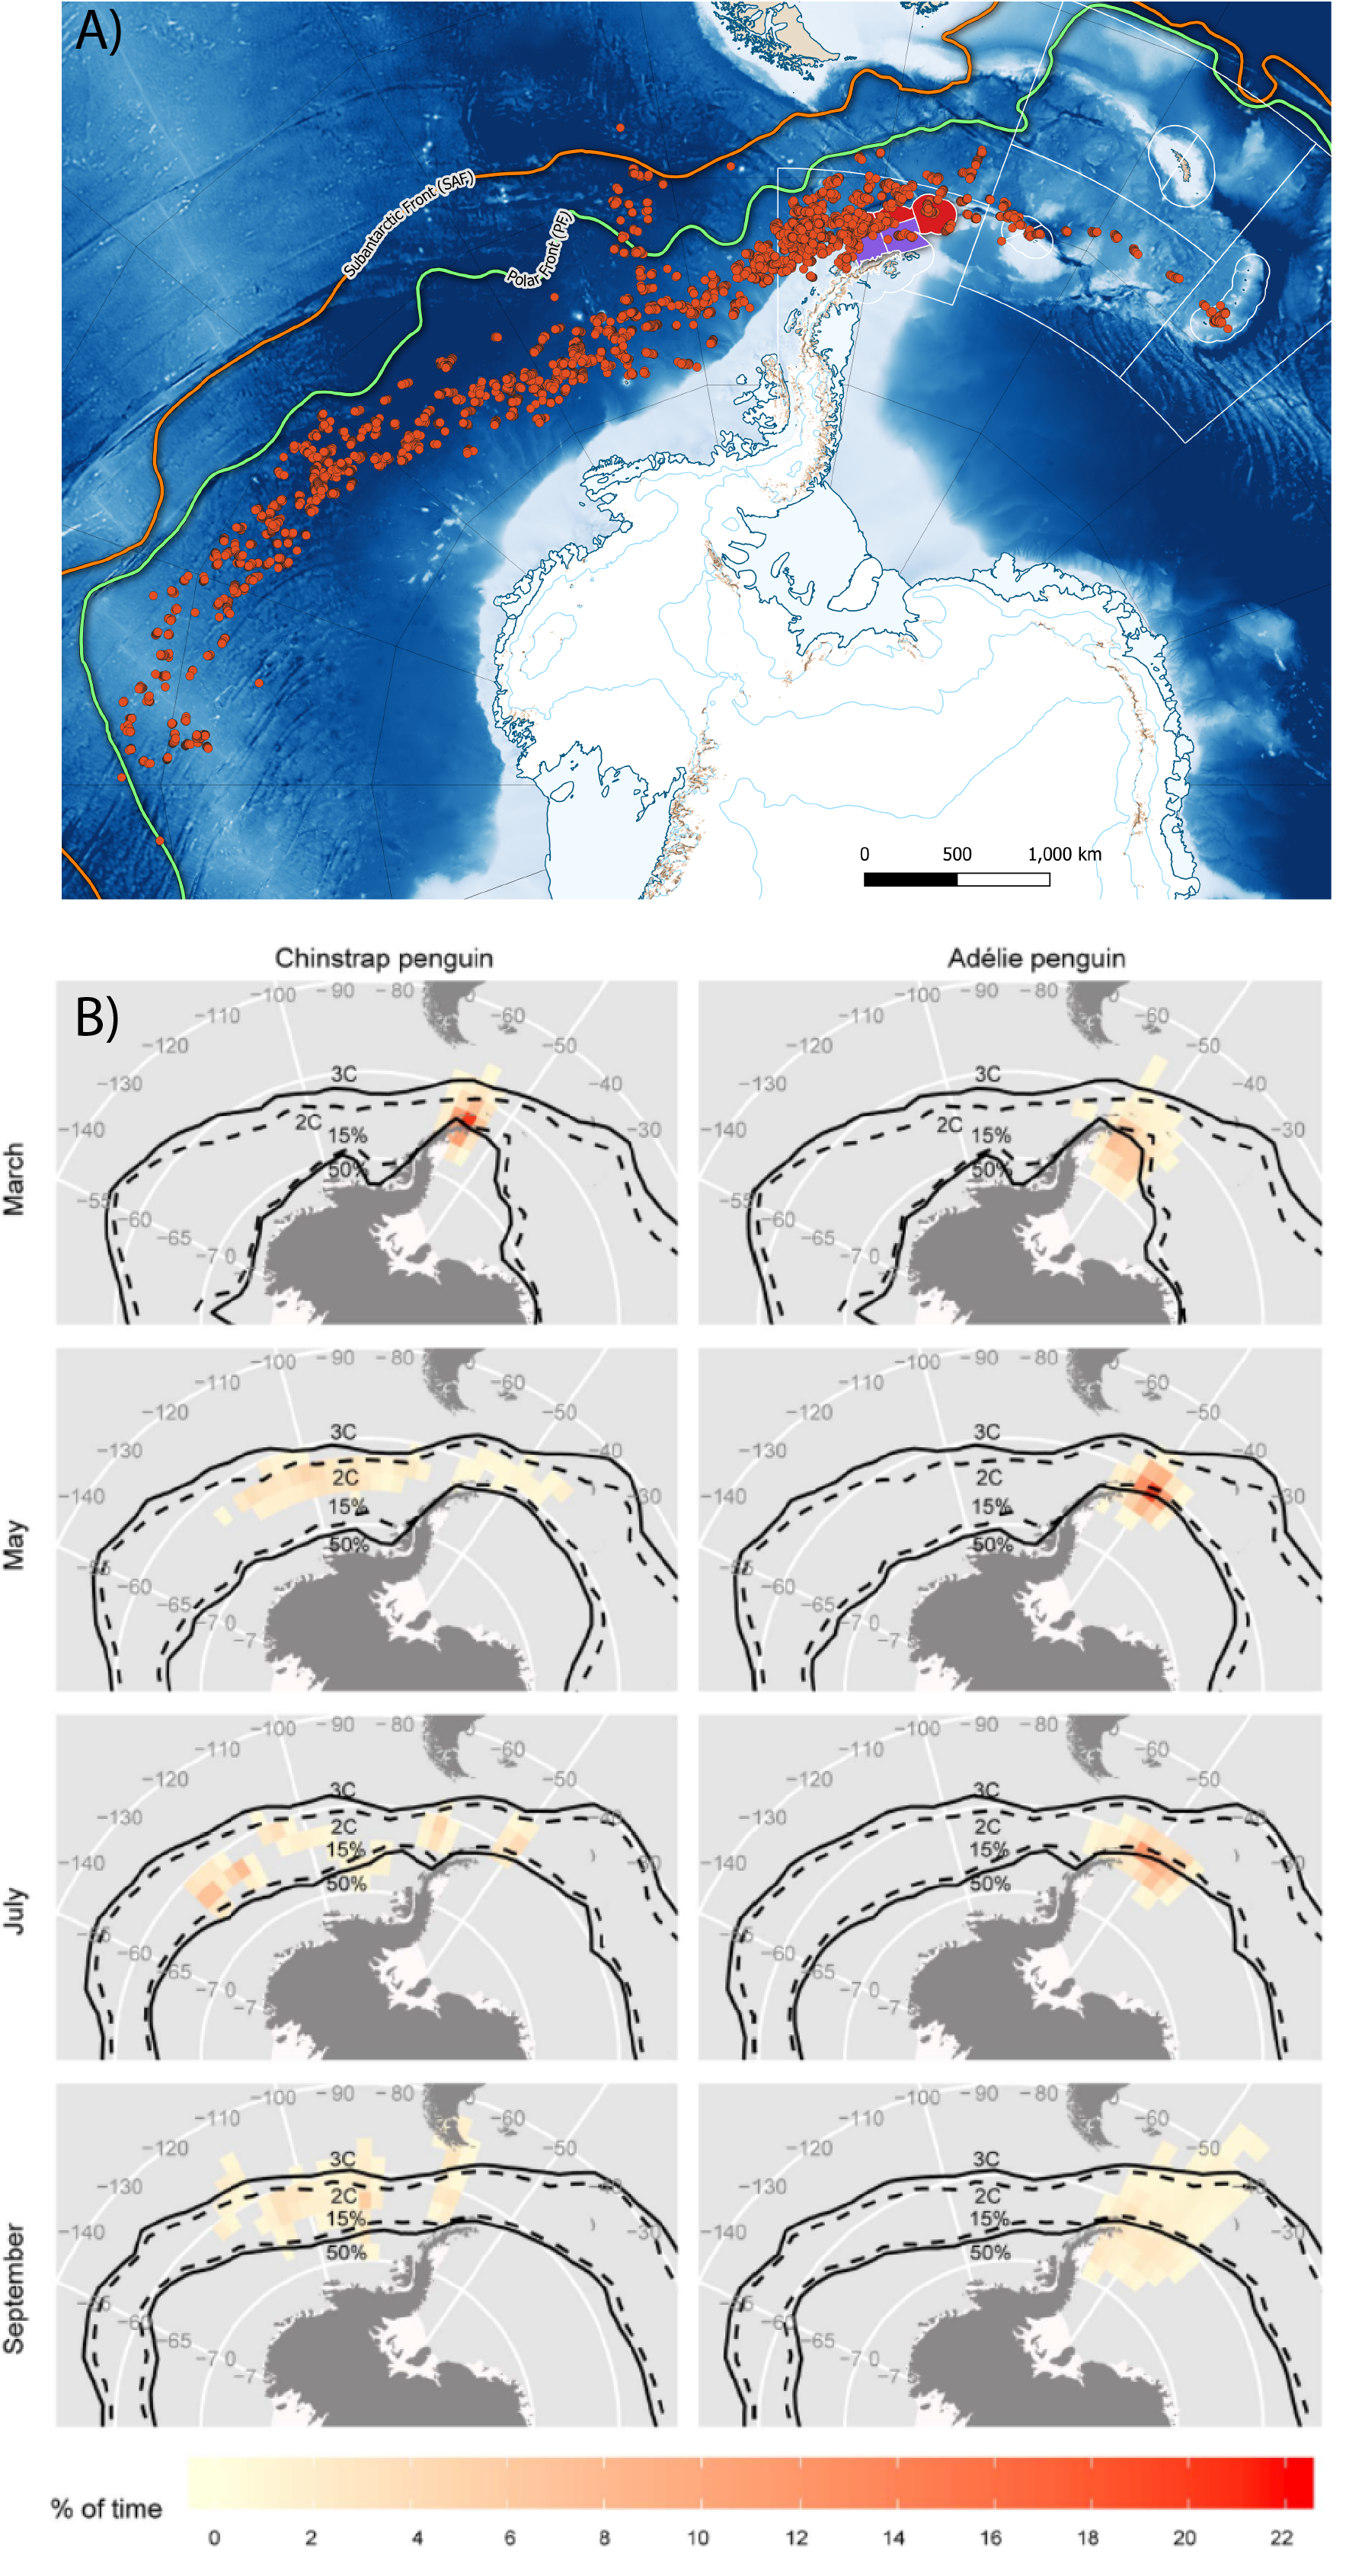
\includegraphics[width=0.75\linewidth]{./Watters EMM figures/Overwinter pengo distributions} \caption{A) Distribution of overwinter movement for chinstrap penguins, relative to the gSSMU's to which they were attributed, created from telemetry data available in Hinke et al. 2019.  B) Adélie and chinstrap penguin movement recorded by light geolocators, highlighting the large longitudinal range both species disperse through at the end of breeding (taken from Hinke et al. 2015).  In the original model formulation by Watters et al. 2020, the winter performance indices for both species are matched to macroscale levels of ONI variability but gSSMU-scale estimates of LKB and LHR.}\label{fig:Overwinter penguin  plots}
\end{figure}

\begin{figure}
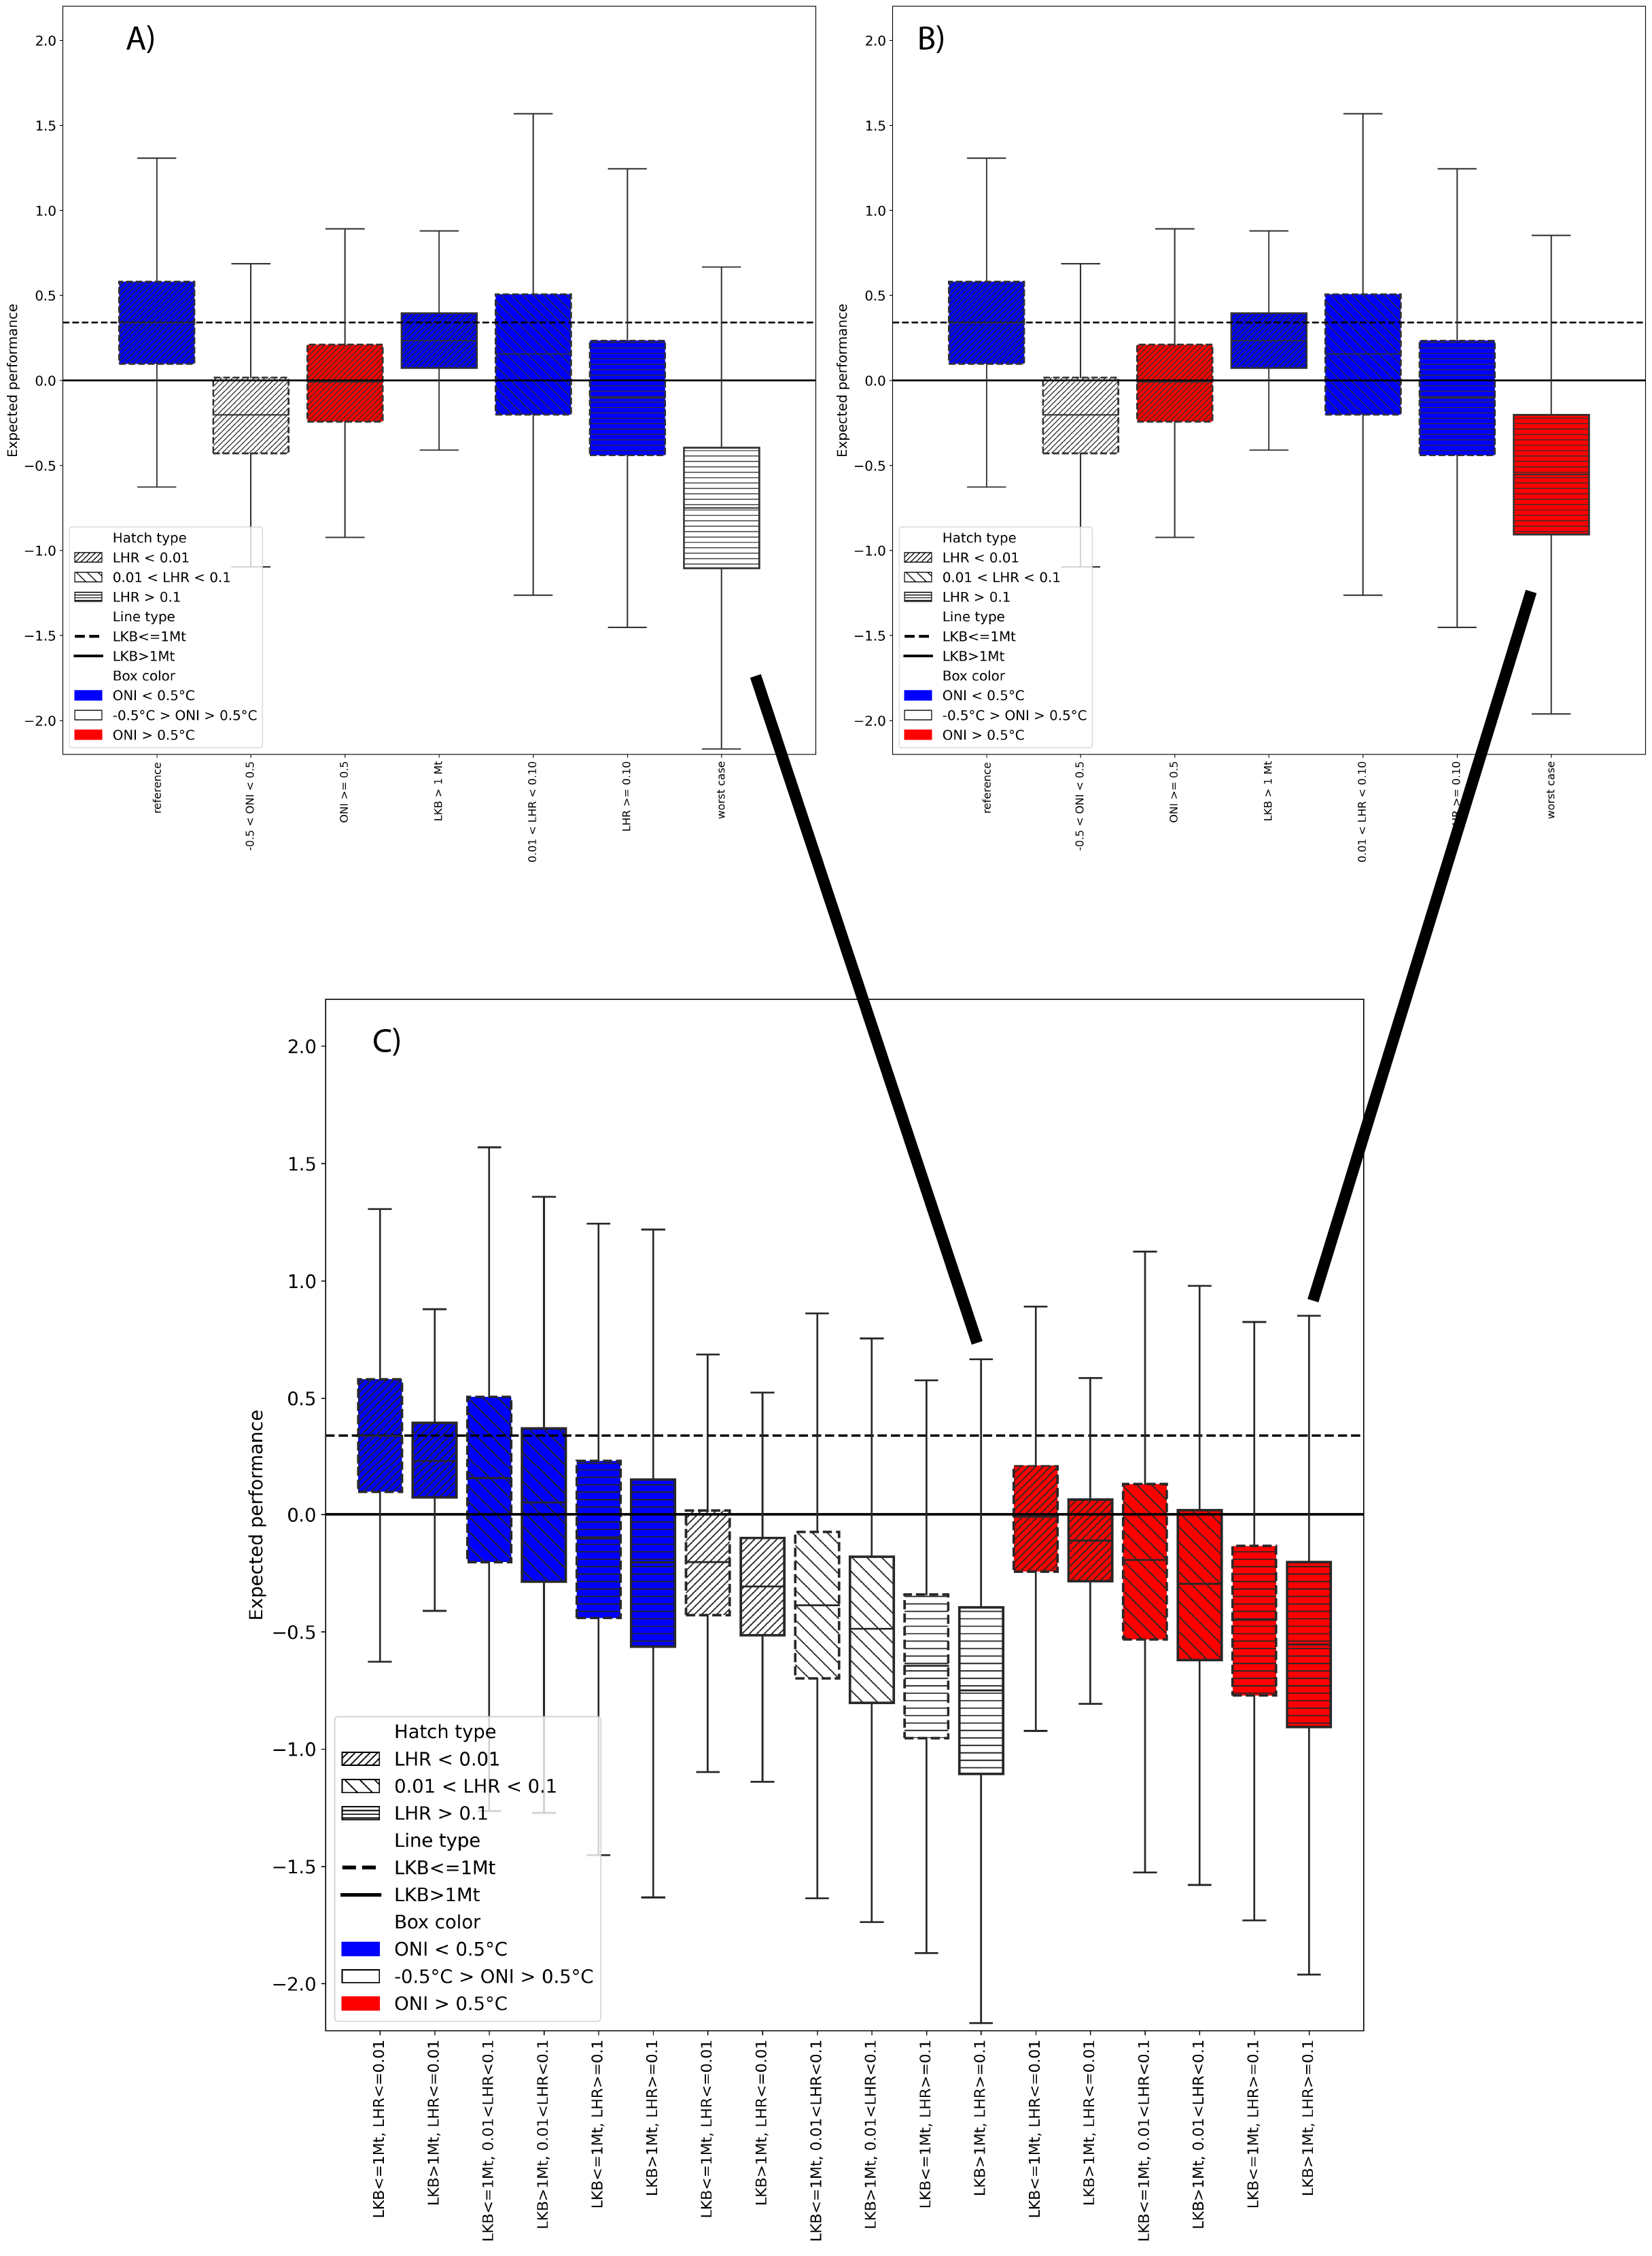
\includegraphics[width=0.75\linewidth]{./Watters EMM figures/Watters original and mistake} \caption{Original Figure 1 plot from Watters et al. 2020 with A) Neutral ONI and B) B) Warm ONI constituting the Worst Case selected.  C) Displays the original case-by-case plots recreated from the paper, with Case 12 representing the intention while data from Case 18 was selected for rendering the boxplot.  Note that the expected performance under neutral ONI Worst Case is poorer than under the warm ONI that was presented in the original paper.  Henceforth, to facilitate comparison, we refer to the ONI Neutral plot however we consider this unrealistic if the intention is to portray a Worst Case of a continuing warming climate.}\label{fig:Watters original and mistake}
\end{figure}

\begin{figure}

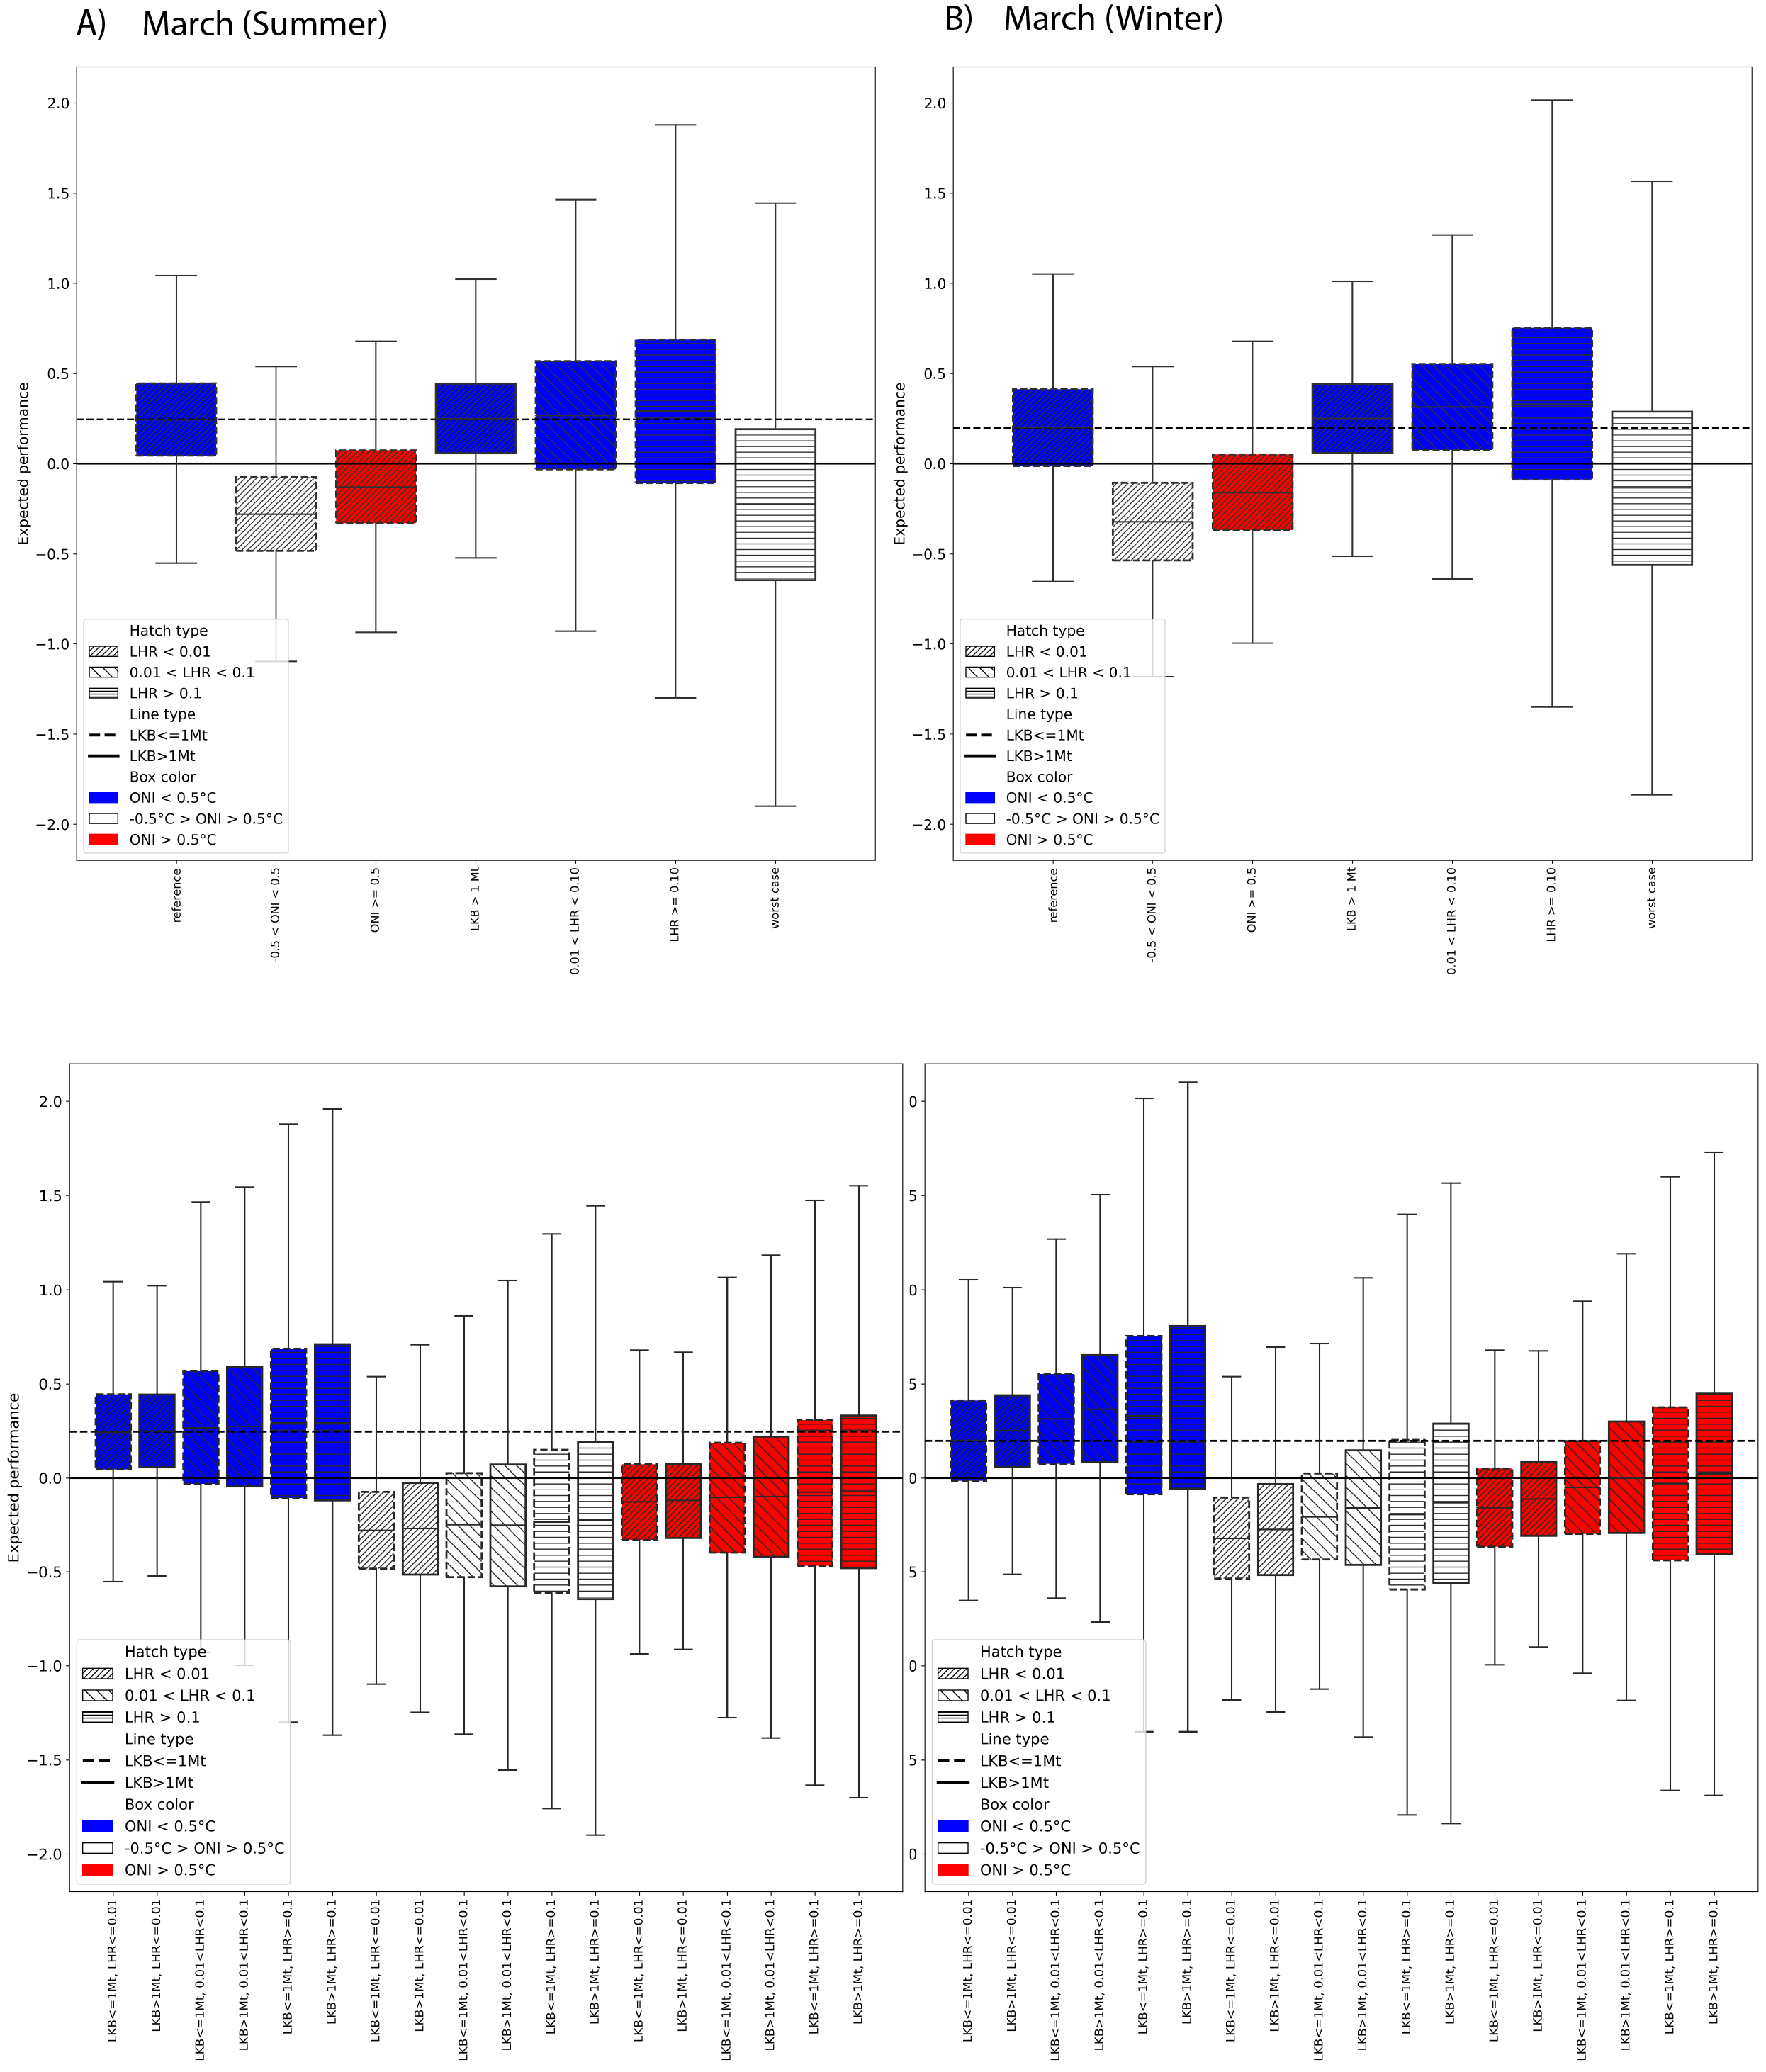
\includegraphics[width=1\linewidth]{./Watters EMM figures/All spp summer then winter 37} \hfill{}

\caption{Model output for the alternatve Watters et al. 2020 scenario outlined above (all species initially present, Adélie and chinstrap penguins migrate out of the area after breeding, LKB and LHR rescaled to SSMU and March included in summer or winter).   Selected cases as per Watters et al. 2020 for March in A) Summer and B) Winter are provided, with the corresponding case-by-case boxplots presented beneath.  Boxplots are colour-coded by ONI state (red=warm, white=neutral, blue=cold).  In all cases, the marginal effect of ONI dominated the expected performance of penguins against their long-term mean, irrespective of LKB or LHR.}\label{fig:Scenario plot 1}
\end{figure}

\pandocbounded{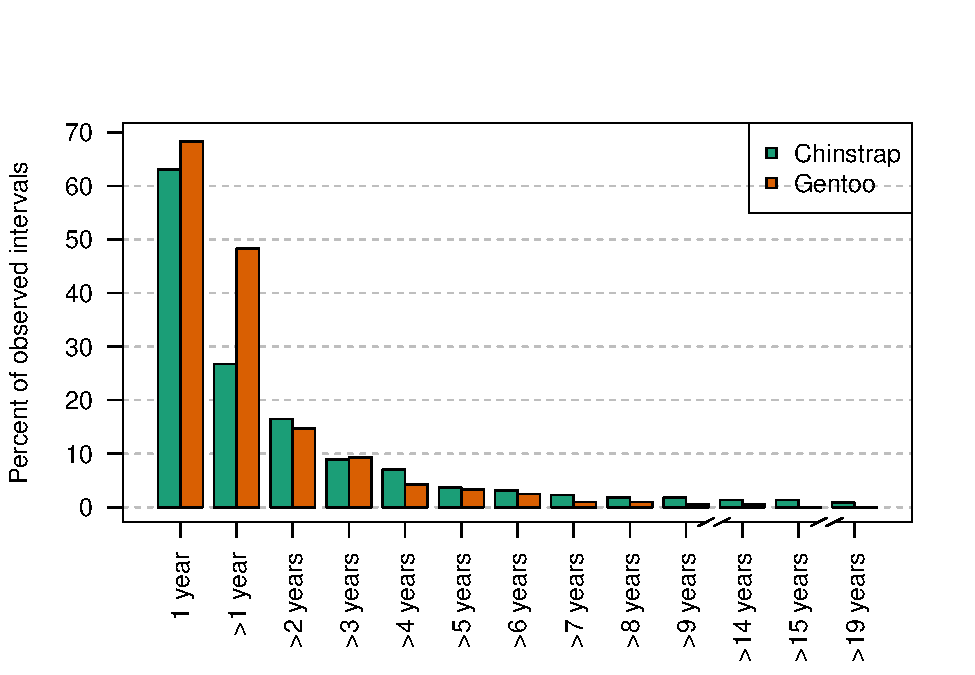
\includegraphics[keepaspectratio,alt={Frequency distribution (percent) of intervals between consecutive breeding surveys for chinstrap and gentoo penguins, taken from the supplementary data for Kruger et al 2021.}]{WattKrug_files/figure-latex/gapCheck-1.pdf}}

\begin{landscape}

\begin{longtable}[t]{lccccc}
\caption{\label{tab:Table 1 Scenario Original}Original table in Watters et al. 2020.  In this and all subsequent tables below, the posterior and posterior predictive probabilities that the expected performance of penguins given the effects in the left hand column are less than the expected performance given the drivers in the column headings are provided. Worst Case is represented by neutral ONI; LHR  $\geqslant$ 0.1; and LKB $\geqslant$ 1Mt.  The Best Case is represented by La Niña conditions, low LKB and low LHR.}\\
\toprule
Effects & Best Case & -0.5 \$\textasciicircum{}\textbackslash{}circ\$ C < ONI < +0.5 \$\textasciicircum{}\textbackslash{}circ\$ C & ONI \$\textbackslash{}geqslant+0.5\$ & Long-term \$\textbackslash{}mu\$ & Long-term predicted \$\textbackslash{}mu\$\\
\midrule
Best case & NA & NA & NA & 0.04 & 0.36\\
ONI Neutral & 1.00 & NA & NA & 0.89 & 0.59\\
ONI warm & 0.99 & NA & NA & 0.52 & 0.51\\
LKB High & 0.71 & 0.02 & 0.12 & 0.01 & 0.41\\
LHR medium & 0.75 & 0.16 & 0.31 & 0.32 & 0.44\\
\addlinespace
LHR high & 0.93 & 0.39 & 0.61 & 0.64 & 0.54\\
Worst case & 0.99 & NA & NA & 0.99 & 0.78\\
\bottomrule
\end{longtable}

\begin{longtable}[t]{lccccc}
\caption{\label{tab:Table 1 Scenario 37a}Posterior and posterior predictive probabilities extracted from the model output for alternatve Watters et al. 2020 scenario outlined above with March attributed to winter (Adélie and chinstrap penguins migrate out of the area after breeding, LKB and LHR rescaled to SSMU). Under this scenario, performance against the long term mean is worst for neutral and warm ONI conditions.}\\
\toprule
Effects & Best Case & -0.5 \$\textasciicircum{}\textbackslash{}circ\$ C < ONI < +0.5 \$\textasciicircum{}\textbackslash{}circ\$ C & ONI \$\textbackslash{}geqslant+0.5\$ & Long-term \$\textbackslash{}mu\$ & Long-term predicted \$\textbackslash{}mu\$\\
\midrule
Best case & NA & NA & NA & 0.04 & 0.40\\
ONI Neutral & 1.00 & NA & NA & 0.97 & 0.62\\
ONI warm & 0.99 & NA & NA & 0.81 & 0.56\\
LKB High & 0.49 & 0.01 & 0.05 & 0.03 & 0.40\\
LHR medium & 0.46 & 0.04 & 0.09 & 0.14 & 0.39\\
\addlinespace
LHR high & 0.45 & 0.10 & 0.16 & 0.23 & 0.39\\
Worst case & 0.84 & NA & NA & 0.71 & 0.59\\
\bottomrule
\end{longtable}

\end{landscape}
\begin{landscape}

\begin{longtable}[t]{lccccc}
\caption{\label{tab:Table 1 Scenario 37b}Posterior and posterior predictive probabilities extracted from the model output for alternatve Watters et al. 2020 scenario outlined above with March attributed to summer (Adélie and chinstrap penguins migrate out of the area after breeding, LKB and LHR rescaled to SSMU). Under this scenario performance against the long term mean is also worst for neutral and warm ONI conditions.}\\
\toprule
Effects & Best Case & -0.5 \$\textasciicircum{}\textbackslash{}circ\$ C < ONI < +0.5 \$\textasciicircum{}\textbackslash{}circ\$ C & ONI \$\textbackslash{}geqslant+0.5\$ & Long-term \$\textbackslash{}mu\$ & Long-term predicted \$\textbackslash{}mu\$\\
\midrule
Best case & NA & NA & NA & 0.10 & 0.42\\
ONI Neutral & 1.00 & NA & NA & 0.98 & 0.63\\
ONI warm & 0.99 & NA & NA & 0.86 & 0.56\\
LKB High & 0.40 & 0.00 & 0.04 & 0.03 & 0.40\\
LHR medium & 0.27 & 0.01 & 0.02 & 0.04 & 0.37\\
\addlinespace
LHR high & 0.37 & 0.08 & 0.13 & 0.21 & 0.38\\
Worst case & 0.76 & NA & NA & 0.63 & 0.55\\
\bottomrule
\end{longtable}

\end{landscape}
\begin{landscape}

\end{landscape}
\begin{landscape}

\end{landscape}

\newpage
\setcounter{table}{0}  \renewcommand{\thetable}{S\arabic{table}}     -   - \setcounter{figure}{0} \renewcommand{\thefigure}{S\arabic{figure}}
\begin{landscape}

\section{Supplementary material}\label{supplementary-material}

\begin{figure}
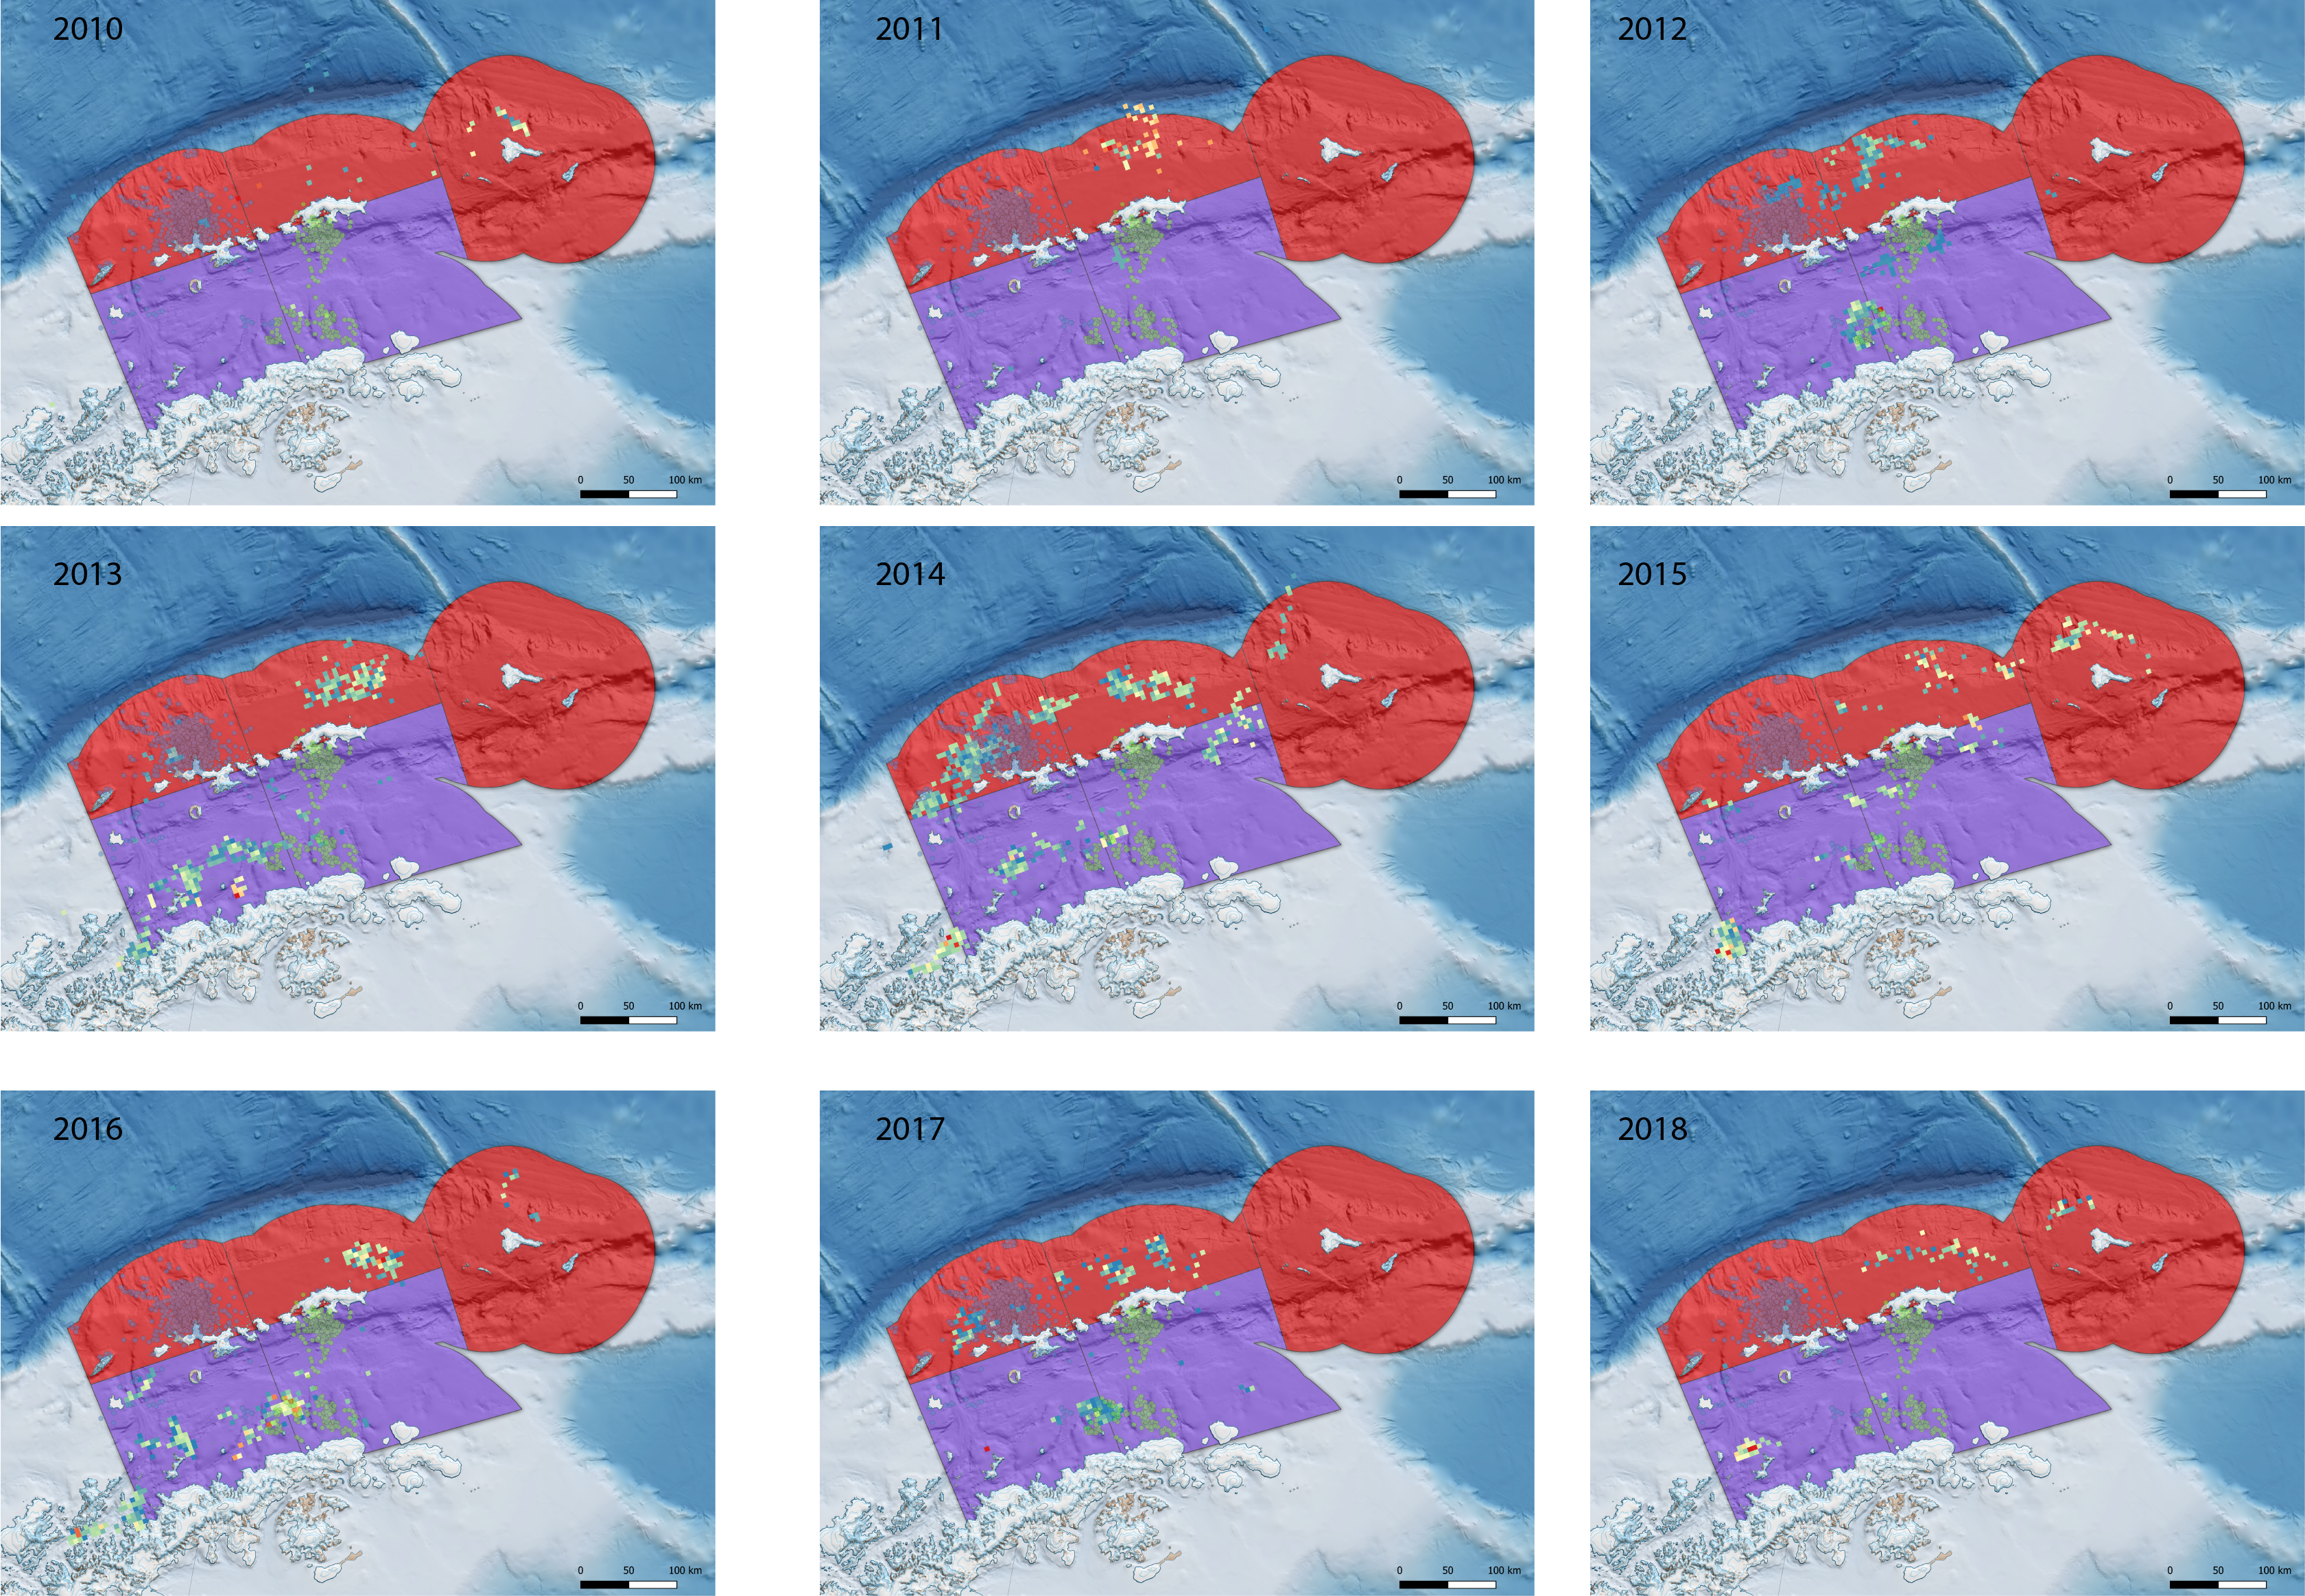
\includegraphics[width=0.8\linewidth]{./Watters EMM figures/summer catch/Year by year catch} \caption{C1 Catch and Effort data for 2010 - 2018, for all catches during the period of the austral summer relating to Adélie and chinstrap penguins in Subarea 48.1 (i.e. up to $10^{th}$ March).  The telemetry data presented in Hinke et al. 2017 for chinstrap penguins at both Cape Shireff and Copacabana and the gSSMU used in the Watters et al. 2020 paper are superimposed to highlight the extreme variability in actual catch, relative to the scale of LHR used to reflect interactions with penguins.  Our reanalysis re-scaled LHR to the SSMU level, though we contend that for the purposes of matching predator data at appropriate spatial scales even this is too coarse a resolution.}\label{fig:Supplementary Figure 1}
\end{figure}

\end{landscape}

\begin{figure}

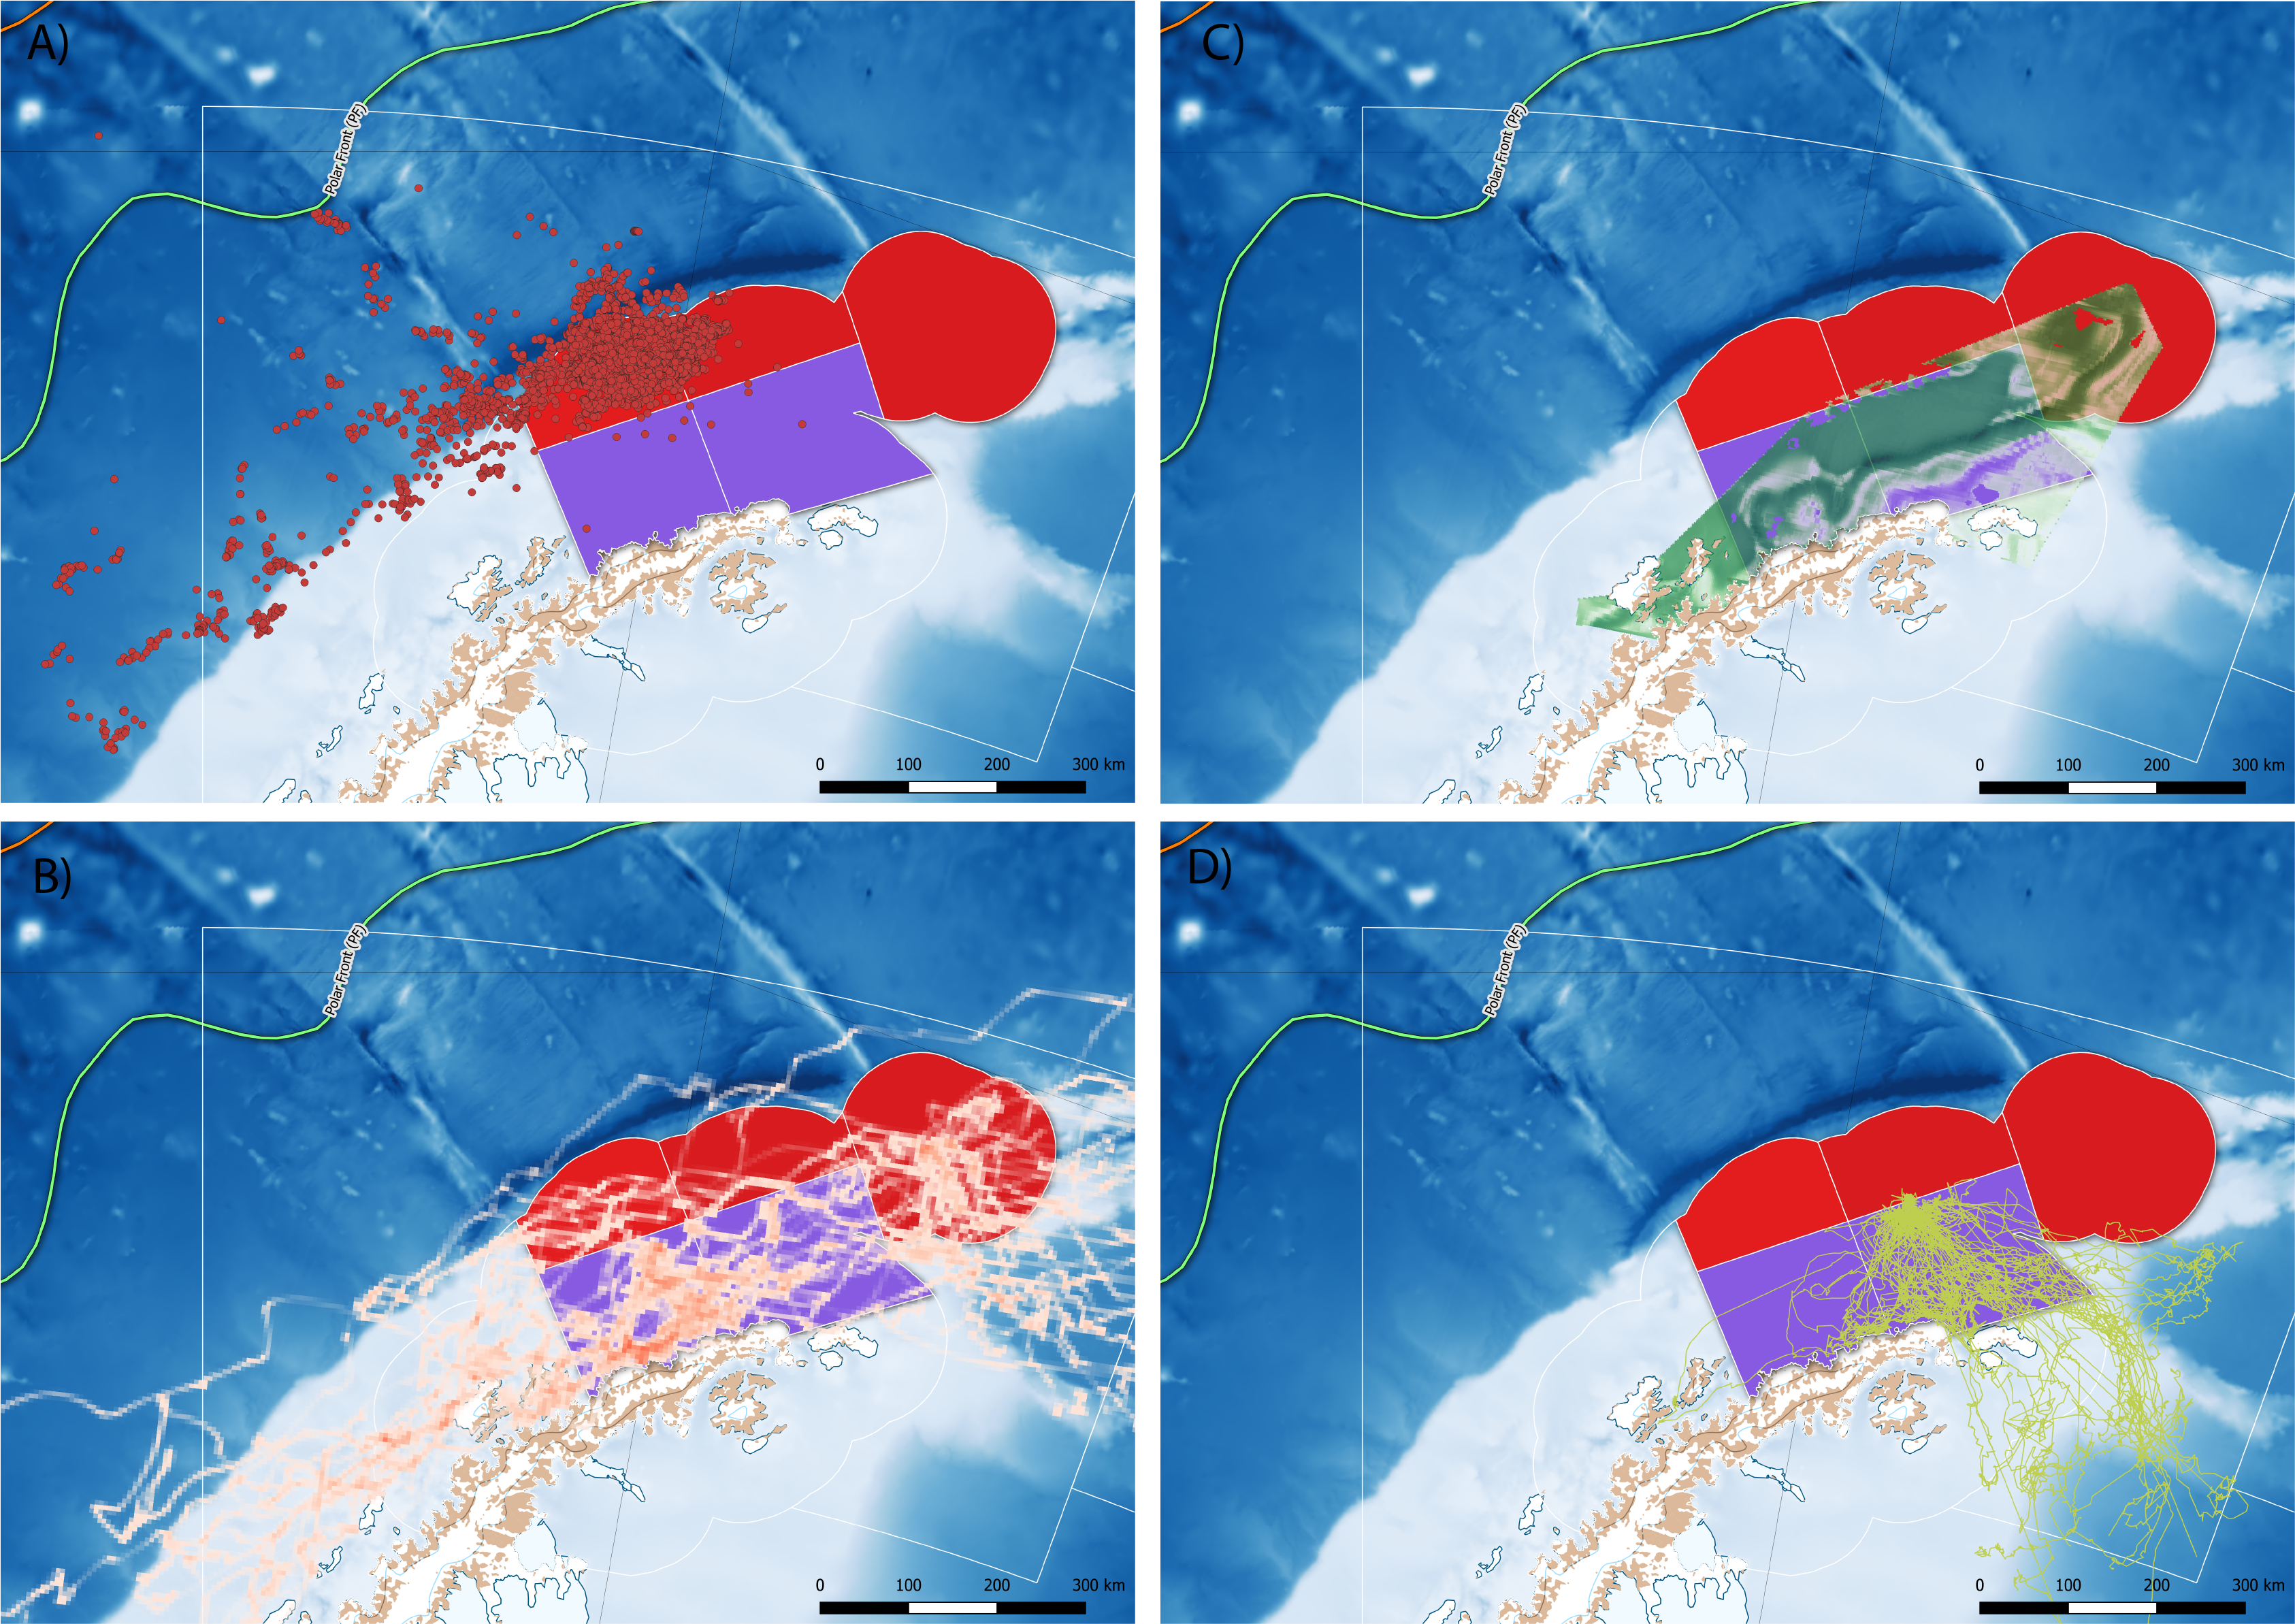
\includegraphics[width=1\linewidth]{./Watters EMM figures/Other spp distribution} \hfill{}

\caption{The summer distribution of foraging effort by A) adult female Antarctic fur seals (adapted from telemetry data available in Hinke et al. 2017), B) migratory adult male Antarctic fur seals (adapted from Lowther et al. 2020) C) humpback whales throughout December (adapted from Johannessen et al., this meeting) and D) nonbreeding adult Adélie penguins during the breeding season (adapted from data in Oosthuizen et al., this meeting). Potential effects of competitive overlap between pygoscelid penguins and other krill dependent predators, particularly those who have increased their abundance dramatically over the preceding 40 years, are excluded from both approaches, creating an unrealistic set of boundary conditions for interpreting the variance in penguin vital rates.}\label{fig:Supplementary Figure 2 other species plots}
\end{figure}

\newpage

\renewcommand\refname{Citations}
\bibliography{mylib.bib}


\end{document}
